\documentclass{report}
\usepackage[utf8]{inputenc}
\usepackage{setspace}
\usepackage[legalpaper, portrait, margin=1in]{geometry}
\usepackage{graphicx}
\graphicspath{ {./images/} }
\usepackage{subfiles}
\usepackage{wrapfig}
\usepackage{caption}
\usepackage{float}
\usepackage{floatflt}
\usepackage{amsmath}
\usepackage{adjustbox}
\usepackage{verbatim}


%--Everything between here and the below cutoff is to maintain R-Code formatting--%

% Options for packages loaded elsewhere
\PassOptionsToPackage{unicode}{hyperref}
\PassOptionsToPackage{hyphens}{url}
\usepackage[hidelinks]{hyperref}  %------- removes red borders - delete this line if necessary
%
\usepackage{amsmath,amssymb}
\usepackage{lmodern}
\usepackage{iftex}
\ifPDFTeX
  \usepackage[T1]{fontenc}
  \usepackage[utf8]{inputenc}
  \usepackage{textcomp} % provide euro and other symbols
\else % if luatex or xetex
  \usepackage{unicode-math}
  \defaultfontfeatures{Scale=MatchLowercase}
  \defaultfontfeatures[\rmfamily]{Ligatures=TeX,Scale=1}
\fi
% Use upquote if available, for straight quotes in verbatim environments
\IfFileExists{upquote.sty}{\usepackage{upquote}}{}
\IfFileExists{microtype.sty}{% use microtype if available
  \usepackage[]{microtype}
  \UseMicrotypeSet[protrusion]{basicmath} % disable protrusion for tt fonts
}{}
\makeatletter
\@ifundefined{KOMAClassName}{% if non-KOMA class
  \IfFileExists{parskip.sty}{%
    \usepackage{parskip}
  }{% else
    \setlength{\parindent}{0pt}
    \setlength{\parskip}{6pt plus 2pt minus 1pt}}
}{% if KOMA class
  \KOMAoptions{parskip=half}}
\makeatother
\usepackage{xcolor}
\usepackage[margin=1in]{geometry}
\usepackage{color}
\usepackage{fancyvrb}
\newcommand{\VerbBar}{|}
\newcommand{\VERB}{\Verb[commandchars=\\\{\}]}
\DefineVerbatimEnvironment{Highlighting}{Verbatim}{commandchars=\\\{\}}
% Add ',fontsize=\small' for more characters per line
\usepackage{framed}
\definecolor{shadecolor}{RGB}{248,248,248}
\newenvironment{Shaded}{\begin{snugshade}}{\end{snugshade}}
\newcommand{\AlertTok}[1]{\textcolor[rgb]{0.94,0.16,0.16}{#1}}
\newcommand{\AnnotationTok}[1]{\textcolor[rgb]{0.56,0.35,0.01}{\textbf{\textit{#1}}}}
\newcommand{\AttributeTok}[1]{\textcolor[rgb]{0.77,0.63,0.00}{#1}}
\newcommand{\BaseNTok}[1]{\textcolor[rgb]{0.00,0.00,0.81}{#1}}
\newcommand{\BuiltInTok}[1]{#1}
\newcommand{\CharTok}[1]{\textcolor[rgb]{0.31,0.60,0.02}{#1}}
\newcommand{\CommentTok}[1]{\textcolor[rgb]{0.56,0.35,0.01}{\textit{#1}}}
\newcommand{\CommentVarTok}[1]{\textcolor[rgb]{0.56,0.35,0.01}{\textbf{\textit{#1}}}}
\newcommand{\ConstantTok}[1]{\textcolor[rgb]{0.00,0.00,0.00}{#1}}
\newcommand{\ControlFlowTok}[1]{\textcolor[rgb]{0.13,0.29,0.53}{\textbf{#1}}}
\newcommand{\DataTypeTok}[1]{\textcolor[rgb]{0.13,0.29,0.53}{#1}}
\newcommand{\DecValTok}[1]{\textcolor[rgb]{0.00,0.00,0.81}{#1}}
\newcommand{\DocumentationTok}[1]{\textcolor[rgb]{0.56,0.35,0.01}{\textbf{\textit{#1}}}}
\newcommand{\ErrorTok}[1]{\textcolor[rgb]{0.64,0.00,0.00}{\textbf{#1}}}
\newcommand{\ExtensionTok}[1]{#1}
\newcommand{\FloatTok}[1]{\textcolor[rgb]{0.00,0.00,0.81}{#1}}
\newcommand{\FunctionTok}[1]{\textcolor[rgb]{0.00,0.00,0.00}{#1}}
\newcommand{\ImportTok}[1]{#1}
\newcommand{\InformationTok}[1]{\textcolor[rgb]{0.56,0.35,0.01}{\textbf{\textit{#1}}}}
\newcommand{\KeywordTok}[1]{\textcolor[rgb]{0.13,0.29,0.53}{\textbf{#1}}}
\newcommand{\NormalTok}[1]{#1}
\newcommand{\OperatorTok}[1]{\textcolor[rgb]{0.81,0.36,0.00}{\textbf{#1}}}
\newcommand{\OtherTok}[1]{\textcolor[rgb]{0.56,0.35,0.01}{#1}}
\newcommand{\PreprocessorTok}[1]{\textcolor[rgb]{0.56,0.35,0.01}{\textit{#1}}}
\newcommand{\RegionMarkerTok}[1]{#1}
\newcommand{\SpecialCharTok}[1]{\textcolor[rgb]{0.00,0.00,0.00}{#1}}
\newcommand{\SpecialStringTok}[1]{\textcolor[rgb]{0.31,0.60,0.02}{#1}}
\newcommand{\StringTok}[1]{\textcolor[rgb]{0.31,0.60,0.02}{#1}}
\newcommand{\VariableTok}[1]{\textcolor[rgb]{0.00,0.00,0.00}{#1}}
\newcommand{\VerbatimStringTok}[1]{\textcolor[rgb]{0.31,0.60,0.02}{#1}}
\newcommand{\WarningTok}[1]{\textcolor[rgb]{0.56,0.35,0.01}{\textbf{\textit{#1}}}}
\usepackage{graphicx}
\makeatletter
\def\maxwidth{\ifdim\Gin@nat@width>\linewidth\linewidth\else\Gin@nat@width\fi}
\def\maxheight{\ifdim\Gin@nat@height>\textheight\textheight\else\Gin@nat@height\fi}
\makeatother
% Scale images if necessary, so that they will not overflow the page
% margins by default, and it is still possible to overwrite the defaults
% using explicit options in \includegraphics[width, height, ...]{}
\setkeys{Gin}{width=\maxwidth,height=\maxheight,keepaspectratio}
% Set default figure placement to htbp
\makeatletter
\def\fps@figure{htbp}
\makeatother
\setlength{\emergencystretch}{3em} % prevent overfull lines
\providecommand{\tightlist}{%
  \setlength{\itemsep}{0pt}\setlength{\parskip}{0pt}}
\setcounter{secnumdepth}{-\maxdimen} % remove section numbering
\newlength{\cslhangindent}
\setlength{\cslhangindent}{1.5em}
\newlength{\csllabelwidth}
\setlength{\csllabelwidth}{3em}
\newlength{\cslentryspacingunit} % times entry-spacing
\setlength{\cslentryspacingunit}{\parskip}
\newenvironment{CSLReferences}[2] % #1 hanging-ident, #2 entry spacing
 {% don't indent paragraphs
  \setlength{\parindent}{0pt}
  % turn on hanging indent if param 1 is 1
  \ifodd #1
  \let\oldpar\par
  \def\par{\hangindent=\cslhangindent\oldpar}
  \fi
  % set entry spacing
  \setlength{\parskip}{#2\cslentryspacingunit}
 }%
 {}
\usepackage{calc}
\newcommand{\CSLBlock}[1]{#1\hfill\break}
\newcommand{\CSLLeftMargin}[1]{\parbox[t]{\csllabelwidth}{#1}}
\newcommand{\CSLRightInline}[1]{\parbox[t]{\linewidth - \csllabelwidth}{#1}\break}
\newcommand{\CSLIndent}[1]{\hspace{\cslhangindent}#1}
\ifLuaTeX
  \usepackage{selnolig}  % disable illegal ligatures
\fi
\IfFileExists{bookmark.sty}{\usepackage{bookmark}}{\usepackage{hyperref}}
\IfFileExists{xurl.sty}{\usepackage{xurl}}{} % add URL line breaks if available
\urlstyle{same} % disable monospaced font for URLs


%--cutoff for R-Code formatting--%



\title{ Bayesian Neural Networks\\

{\large A Thesis \\
Presented to the Faculty of the  \\
Department of Mathematics \\
West Chester University  \\
West Chester, Pennsylvania  \\
  

In Partial Fulfillment of the Requirements for the Degree of \\
Master of Science in Applied Statistics \\


By  \\

}}


\author{Samuel Richards}
\date{May 2023}


\begin{document}

\begin{spacing}{2.5}
\maketitle
\end{spacing}


%\chapter*{Dedication}
%(optional)

%	The dedication page is an optional page where you can dedicate the master’s thesis/doctoral culminating project at your discretion.  


%\chapter*{Acknowledgements}
%The acknowledgment page is an opportunity to recognize those who supported you in various capacities throughout the master’s thesis/doctoral culminating project. The chair, committee members, family members, friends, colleagues, and/or anyone you wish to recognize are often mentioned here. 

\chapter*{Abstract}
Inspired by the mechanics of brain functionality, artificial neural networks (ANN’s) are powerful statistical models that capture complex trends in data.  These models incorporate a series of algorithms that compete with error functions to adjust their parameters based on some training data.  Because of their immense complexity, with hidden layers operating like a black box, traditional neural networks require a lot of training data in order to produce viable results.  It’s not uncommon for a neural net to have several thousand or millions of parameters, each a tiny knob that needs to be fine-tuned precisely.  This makes ANN’s so flexible during training that they can become overfit to the data that trained them and thus less practical in application.  In addition, their architecture puts a lot of trust in the algorithms that comprise them and makes it difficult to measure uncertainty in their predictions.  While regularization techniques such as dropout and weight decay address these issues, constructing a network from a Bayesian approach offers another solution, particularly in short supply of data.  Bayesian neural networks, which use the entire posterior distribution rather than a single parameter estimate, are models with a means of describing this uncertainty with more transparency.  A parameter of a BNN has a measure of belief in its value through a posterior distribution, which allows for the same input to yield slightly varying results based on the likelihood of the output.  The result is a powerful and adaptive model, with a built-in means of describing its accuracy and the capacity to learn from a small amount of data.

\tableofcontents

\chapter{Introduction to Deep Learning}

Artificial intelligence is the start to outsourcing brain function to man-made machines.  A machine is said to have "Artificial Intelligence" if it can do what people say requires intelligence \cite{jackson2019introduction}, from counting monetary denominations to surveying Mars, playing chess games to converting human speech.  Within the realm of this is the subcategory known as machine learning, in which models are tested based on training data in order to "teach" them right from wrong.  Machine learning has an increased emphasis on the use of computers in statistical analyses and a decreased emphasis on proving confidence intervals around them \cite{Goodfellow-et-al-2016}.  With astronomical advances in modern computing technology, creating elaborate learning models with raised functionality has become more and more accessible, creating a new category known as deep learning, which is the parent of the subjects within this thesis.  Deep learning models operate beyond those of traditional machine learning as such models contain layers of complexities, each performing a specific task for the overall objective.  Algorithms and procedures unite with complex mathematical formulas to generate extremely precise models without the assumptions of linear models.

%---EXAMPLE FOR PHOTOS--
%--- https://www.overleaf.com/learn/latex/Inserting_Images ---for reference
\begin{figure}[h]
    \centering
    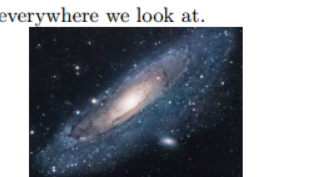
\includegraphics[width=0.25\textwidth]{poo}
    \caption{a nice plot}
    \label{fig:mesh1}
\end{figure}

\section{What is Deep Learning?} %-------------SECTION

Deep learning is the brand of machine learning concerned with using Artificial Neural Networks to reveal complex abstractions within data.
The evolution of the process of mimicking cognitive brain functionality within artificial machines dates back to the 1940's under the term cybernetics, which was originally intended to provide computational models for biological understanding \cite{Goodfellow-et-al-2016}.  Since then, the history of what we now call "deep learning" has undergone waves of renaissance.

\subsection{Working with Structured Data} %-------------SECTION

\subsection{Working with Unstructured Data} %-------------SECTION


\chapter{Artificial Neural Networks}
Introduce ANN's more specifically here.

\section{The Architecture of Neural Networks} %-------------SECTION
This will primarily be the \textbf{BabyNeuralNet.rmd} file.

This section will be RICH in \textbf{mathematical notation}
Hint toward issues like overfitting, but elaborate more in section 2.3.

- Also, first mention \textbf{Optimization} here

\subfile{Architecture}  % Pathway to BabyNeuralNet file

%\subsection{Gradient Descent}

%\subsubsection{Simulation in R}

%\subsection{Backpropagation}

%\subsubsection{Simulation in R}

\subsection{More Optimization Algorithms and Activation Functions}

\section{Types of Neural Networks} %-------------SECTION

Write this up in R following along the code from \textbf{RAI}, with supplementary information from other sources as well.  

Obviously not all types will be covered, but here are a few.  

Include \textbf{mathematical notation} for each network mentioned.

\subsection{Multi-Layer Perceptron}
Keras Model: "sequential"

\subsection{Convolutional Neural Networks}
Unstructured image data

\subsection{Generative Adversarial Networks}
Unstructured image data

\subsection{Recurrent Neural Networks}
Unstructured text data

\subsection{Long Short-Term Memory Network}
Unstructured text data

\subsection{Convolutional Recurrent Networks}
Unstructured text data

\section{Techniques to Improve Model Performance} %-------------SECTION

The primary objective in machine learning (and therefore deep learning) is to perform well on new, unseen data. 

- \textbf{Overfitting} and \textbf{underfitting}

\subsection{Rating Model Performance}
- \textbf{Generalization}
- \textbf{Training error}  
- \textbf{Generalization error} (test error)

\subsection{Addressing Model Performance}
- \textbf{Capacity}
- \textbf{Regularization}

\subsection{Common Problems and Relevant Techniques}

Earthquake example

\chapter{Bayesian Statistical Methods}

Brief description, background, difference (NOT opposition) from frequentist statistics.

The frequentist approach describes probability as the relative frequency of a favorable outcome as the number of samples increases to infinity.  In Bayes, probability is the number of favorable outcomes divided by the total number of possible outcomes \cite{gelmanbayesian3}
$$
P = \frac{N_{\text{favorable outcomes}}}{N_{\text{total possible outcomes}}}
$$

\textit{(add these into the intro paragraph)}
\begin{itemize}
\tightlist
\item
Pros: usable information with little data
\item
cons: computationally intensive or impossible
\end{itemize}


\section{Fundamentals of Bayesian Inference} %-------------SECTION

\textit{(theoretical representations)}

A few things change when operating with the Bayesian framework.  For one, the goal is not to construct a model to estimate parameters as fixed values.  Rather, parameters are treated as random variables themselves, with the same properties as any other random variable - each could have a mean, a variance, minimum maximum, etc., and the distribution of that parameter reveals that information.

Exact Bayesian inference

$$
p(w|D) = \frac{p(D|w)p(w)}{p(D)} = \frac{p(D|w)p(w)}{\int_{w'} p(D|w')p(w')dw'}
$$


\subsection{From Prior to Posterior}

Selection of priors, perhaps advise on broad priors that tell little information.

Hand calculation of a Gaussian prior to compute a posterior to be used in a later section
%prior to posterior involves using MLE and the prior as we have done before in 506  Use my notes from then to compute a posterior distribution for a Gaussian prior


\subsection{Bayesian Updating}

Bayesian updating, in which the posterior is the new prior

$$
pretty ggplot display here
$$

\textit{Address computational issues like the normalizing constant, to be discussed further in the next section.}

\section{Practical Computing}



 As mentioned, the premier disadvantage of Bayesian inference is that is requires computationally intractable integrations.  In response, a world of practical approximation techniques exists, some of which will be discussed in this section.  These approximaton techniques can be shown to still have pristine results while dodging tricky or impossible integrals \cite{tipping2004bayesian}.

 Approximate Bayesian inference

$$
p(w|D) \approx \frac{p(D|w)p(w)}{Z}
$$
In which $Z$ is approximated by some sophisticated means.

 mention other approximation techniques from Rethinking like Laplace and Grid (lecture 8 notes and referenced book pages)


\subsection{Markov Chain Methods}
Used to address the problem of highly complex integral
\textit{(To be expanded into multiple subsections)}

Start with:
\cite{mcelreath2016statistical} \cite{gelmanbayesian3}
\begin{itemize}
\tightlist
\item Overview
\item Metropolis (Rosenbluth) Algorithm
\item M-H Algorithms
\item Gibbs Sampling \cite{geman1984stochastic}
\item MCMC
\item Computationally efficient versions
\end{itemize}

\textit{(Relevant examples in STAN whenever appropriate)}


\section{Bayesian Data Analysis} %-------------SECTION

\textit{(More practical representations)}

This section focuses on more tools in the Bayesian framework

\subsection{Marginalization}

Introduce marginalization to integrate unwanted parameters. (Occam's Razor things)

Construct notation by following along from 
\cite{tipping2004bayesian} and page 165 of \cite{bishop2006pattern}

Posterior Inference given (introduce the notational terms)
$$
Tipping p. 14
$$

Integrate out unwanted parameters for the \textit{predictive distribution} of a new data $t_*$:
$$
p(t_*|t,\alpha,\sigma^2) = \int p(t_*|w,\sigma^2) p(w|t,\alpha,\sigma^2) dw
$$

Where  $p(w|t,\alpha,\sigma^2)$ is the posterior distribution and $p(t_*|w,\sigma^2)$ is the likelihood of the new data.  If $w$ and $\sigma^2$ were known to be true, then the likelihood would determine the prediction for future data.  Since these are unknown, and because under Bayes parameters are random variables, the predictive distribution is a weighted average over the posterior.  Thus, the  predictive distribution can be interpreted as the expectation of the single network likelihood under the posterior $p(w|t,\alpha,\sigma^2)$. \cite{salad}


In the absence of many data points, the predictive distribution will be very sparse. \cite{tipping2004bayesian}


\textbf{Simulating the Predictive Distribution}
$$
Insert Simulationhere
$$

Ideally, to be fully Bayesian and practice the mastery of marginalization is to integrate out \textit{all} variables that are not related to the task at hand. \cite{bishop2006pattern}.

Full posterior:
$$
p(w,\alpha,\sigma^2|t) = \frac{p(t|w,\sigma^2) p(w|\alpha)p(\alpha)p(\sigma^2)}{\iiint p(t|w,\sigma^2)p(w|\alpha)p(\alpha)p(\sigma^2) \text{ } dw \text{ } d\alpha \text{ } d\sigma^2}
$$





\subsection{Predictive Accuracy Measures}
I feel I need to put Bayes-CV somewhere...

Mention of their frequentist analog (for lppd is is the log-probability score on Rethinking p. 214)

\textbf{Bayesian Cross-Validation} to get the log-pointwise predictive density
$$
lppd_{CV} = \sum_{i=1}^N \frac{1}{S} \sum_{s=1}^S logP(w_i|\theta_{-i,s})
$$

\textbf{Information Criteria} also found in Rethinking (p. 223) and BDA (p. 169)


\subsection{Bayesian Regularization}


The first chapter of this thesis described weight decay as a regularization technique.  Recall it left with the following full-optimization formula:

$$
F = \alpha E_W(w|A) + \beta E_D(D|w,A)
$$



This section will apply a Bayesian Approach to setting $\alpha$ and $\beta$ parameters, as told by (Mackay, 1992) \cite{mackay1992practical} and (Forsee and Hagan, 1997). \cite{foresee1997gauss}

The weights of the network as random variables. By Bayes' rule:
 
$$
P(w|D,\alpha,\beta,A) = \frac{P(D|w,\beta,A) P(w|\alpha,A)}{P(D|\alpha,\beta,A)}
$$

where $D$ is the observed data, and $A$ is the network architecture.\footnote{
\textcolor{darkgray}{
Note that (Mackay, 1992) defines a term $R$ as the chosen or "prior" regularizer, which represents the potential for selecting alternative control parameters for for $E_W$.  If included, Bayes' rule would then be represented  as:
$$
P(w|D,\alpha,\beta,A,R) = \frac{P(D|w,\beta,A,R) P(w|\alpha,A,R)}{P(D|\alpha,\beta,A,R)}
$$
 and subsequent formulation would be modified to represent $R$. However, this example only considers the sums of squares regularizer $E_W$ from chapter 1 and so the extended notation has been be omitted for this thesis.
 }}
Taking into assumption that the model residuals follow a normal distribution, the likelihood function \cite{foresee1997gauss}, representing the probability of the data given weights $w$, is
$$
P(D|w,\beta,A) = \frac{1}{Z_D(\beta)} e^{-\beta E_D}
$$
and by establishing the prior distribution as normal, its density is represented as:
$$
P(w|\alpha,A) = \frac{1}{Z_W(\alpha)} e^{-\alpha E_W}
$$
for which
$$
Z_D(\beta) = \left( \frac{\pi}{\beta} \right) ^{n/2} \text{ and }
Z_W(\alpha) = \left( \frac{\pi}{\alpha} \right) ^{N/2}
$$

Putting this all together, the posterior distribution can be represented as:
$$
P(w|D,\alpha,\beta,A) = \frac{\frac{1}{Z_W(\alpha)} \frac{1}{Z_D(\beta)} e^{-(\beta E_D + \alpha E_W)}}{P(D|\alpha,\beta,A)} \\
= \frac{e^{-(\beta E_D + \alpha E_W)}}{Z_F(\alpha,\beta)}
$$

Thus it can be noted by the formula above that under Bayes, the optimal weights should maximize the posterior probability, which is equivalent to minimizing the full optimization formula $F = \alpha E_w(w|A) + \beta E_D(D|w,A)$ as seen in chapter 1.  For later use, the normalizing constant in the denominator is $Z_F(\alpha,\beta) = \int d^k w e^{-(\alpha E_W + \beta E_D)}$.


\textbf{Optimizing the Regularization Parameters}

By use of Bayes' rule, the posterior probability for the parameters $\alpha$ and $\beta$ is:

$$
P(\alpha, \beta | D,A) = \frac{P(D|\alpha,\beta,A) P(\alpha,\beta)}{P(D|A)}
$$



Suppose a uniform prior is chosen for ($\alpha,\beta$).  By this, the posterior distribution would be maximized by maximizing the \textit{likelihood} function.  What's more is that the likelihood function is the normalizing constant above.  With algebra, and by maintaining the previous assumptions, the likelihood function would take the form:
$$
P(D|\alpha,\beta,A) = \frac{P(D|w,\beta,A) P(w|\alpha,A)}{P(w|D,\alpha,\beta,A)}
$$
and since the heavy integration of the normalizing constant is already simplified, this equation can be computed.
$$
\frac{\frac{1}{Z_W(\alpha)} \frac{1}{Z_D(\beta)} e^{-(\beta E_D + \alpha E_W)}}{\frac{1}{Z_F(\alpha,\beta)} e^{-F(w)}} = \frac{Z_F(\alpha,\beta)}{Z_D(\beta) Z_W(\alpha)} \cdot \frac{e^{-(\beta E_D + \alpha E_W)}}{e^{-F(w)}} = \frac{Z_F(\alpha,\beta)}{Z_D(\beta) Z_W(\alpha)}
$$

The denominator is comprised of known constants $Z_D(\beta)$ and $Z_W(\alpha)$.  What is left is to determine $Z_F(\alpha,\beta)$.  Having outlined the Bayesian techniques, this thesis will not cover this decomposition.  In practice, it requires estimation by Taylor series expansion and computation of the Hessian matrix of the full optimization formula $H = \beta \nabla^ E_D + \alpha \nabla^2 E_W$ to determine the number of effective parameters in the neural network that are reducing the error function.  This decomposition can be found in (Mackay, 1992) and (Forsee and Hagan, 1997).


\begin{comment}
Through \textbf{margialization}, the true posterior $P(w|D,A)$ is obtained by integrating out $\alpha$ and $\beta$:
$$
P(w|D,A) = \int P(w|D,\alpha,\beta,A) P(\alpha, \beta | D,A) \text{ } d\alpha \text{ } d\beta
$$
\end{comment}

\subsection{Example: Bayesian Regularized Neural Network}

Introduce the brnn package



\chapter{Bayesian Neural Networks}

\begin{wrapfigure}{r}{0.3\textwidth}
  \vspace{-40pt}
    \centering
    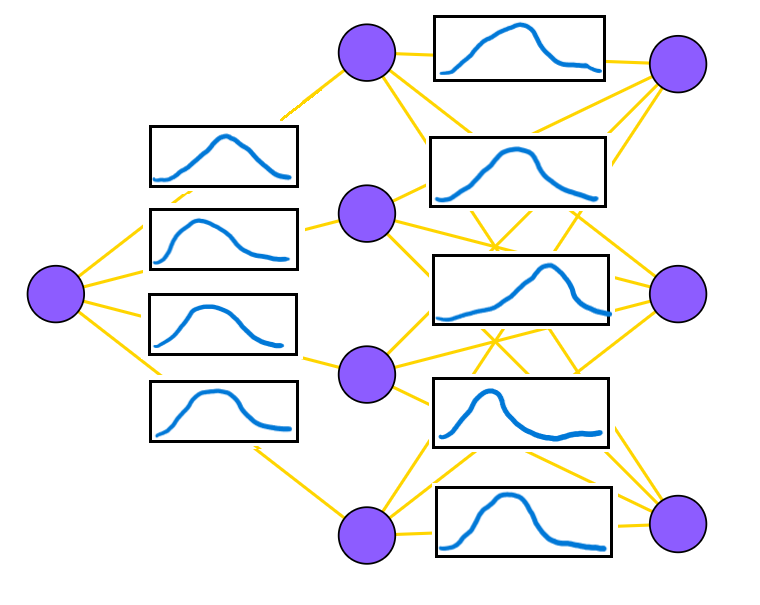
\includegraphics[width=.35\textwidth]{Figures/BNN_weightstoc.png}
    \caption{\footnotesize{A two-layer Bayesian Neural Network with parameters as distributions rather than strict point estimates.}}
  \label{BayesNet}
  \vspace{-10pt}
\end{wrapfigure}

 In the ``traditional'' neural network framework, to train a neural network to minimize its error based on a single point estimate for each $w_i$, waged against a cost function, is to maximize the likelihood of the training data (i.e. finding weights $w_i$ that maximize $P(D_{train}|W)$ \cite{bishop1995} \cite{bishop1997bayesian}.  The drawback to an ANN is that the distribution of network parameters $\theta = (W,b)$ across the network is unknown. \cite{mullachery2018bayesian}  Without supplemental engineering, measurements of the model's uncertainty cannot be quantified (as described earlier).
 
 In Bayes, there are no point estimates. Instead, by use of Bayes’ Rule, an interval of potential weights based on probabilities $p(w|D)$ is computed.  As such, the network can express uncertainty in its weights through this posterior distribution.  What's more is by the rudimentary feature of marginalization, uncertainty can be quantified for the predicted outputs $p(y|D)$ (for either $y$ as a regression prediction or classification label); even the very architecture of the model $p(A|D)$ can be expressed as a distribution. \cite{bishop1995}
 

\section{Architecture}

A researcher unsatisfied with a single point estimate for network outputs may consider simulating multiple networks, introducing a stochastic effect to parameter tuning so as to not generate the same results. Stochastic neural networks, which use either stochastic activations or stochastic weights, simulate multiple possible models $\theta$ with associated probability distribution $p(\theta)$.  Aggregating independent predictors can lead to better predictions than single point estimates. \cite{Jospin}.  In comparing the predictions of multiple samples of $\theta$, stochastic models better measure uncertainty.  Bayesian neural networks are a special case of stochastic neural networks in which the ensemble of possible models is obtained using Bayesian inference. \cite{mackay1992practical}

\subsection{Stochastic Modeling} B
JOSPIN, page 5

Stochastic neural networks are ANN's with a stochastic element introduced into the model.  A simple example is the regularization technique dropout \cite{goan2020bayesian} described earlier.  A neural network trained with dropout has a component randomness introduced by the selection of neurons removed from training.  If the dropout model was trained over and over again, it would contain slightly different parameter values reflective of this random noise.  There are other ways to introduce stochasticity into the model.  For example in regression, the network could assume residual normality by introducing Gaussian noise in its data generation \cite{Jospin}.  That is, for parameterizing weights $w$:
\begin{gather*}
\theta \sim N(\mu,\sigma^2) \\
w \sim p(w|D_{train},\theta)
\end{gather*}

This is the essence of how a BNN is a special case of a stochastic model.  The difference lies in that the stochastic element $\theta$ lies in the prior $p(\theta)$.

\subsection{Selection of Priors}

\textit{(Refer back to "From Prior to Posterior" and reiterate how to select priors for BNN's, specifically)}

There is no one-size-fits-all for machine learning models, and deep learning models only inflate this fact due to their enormous complexity \cite{Goodfellow-et-al-2016}.  Therefore, it can be interpreted \cite{Jospin} that prior assumptions are in place for all machine learning models, be it the optimization algorithm, regularizer, architecture, etc. These are implicit for non-Bayesian networks.  However, with Bayes, the prior assumptions are made explicit.  Yet, by the same logic, it is not always intuitive how to select priors.  A beginner's start for a regression task is to select a normal prior $p(\theta) \sim N(\mu,\sigma^2)$.  This is analogous to the point-estimate weight decay regularization described in earlier sections, but will be further discussed later in this section. \textbf{DO THIS and ensure the same notation}  Despite this, there is no theoretical argument that makes a normal prior better than any other \cite{silvestro2020prior}; it simply has nice mathematical properties.


\subsection{Development}

\textit{(Add more here.  Introduce the prior selected from the last subsection and incorporate more steps to reaching the posterior)}

Recall that $\theta$ represents the model weights and biases $(W,b)$.  $D$ is the training data from which the model learns, its inputs and outputs denoted with sibscripts $_x$ and $_y$.  Applying Bayes' Theorem, to determine the posterior distribution of $\theta$ requires selection of a prior and determination of the likelihood of the data:

$$
p(\theta|D) = \frac{p(D_{y}|D_{x},\theta)p(\theta)}{\int_\theta p(D_{y}|D_{x},\theta')p(\theta')d\theta'}
$$

The normalizing constant in the denominator is what has been seen before: the difficult (profoundly intractable for any informative BNN's) integral that requires estimation by Markov Chain Monte Carlo or variational inference.

\textit{(lead into the next subsection)}

\subsection{Inference}

\textit{(Add more into this section.  Check a reference, first, to see what I can add...)}

Marginalization takes reign when determining the distribution of network predictions.  This means integrating out $\theta$ from the final model.  Given the posterior distribution of network parameters $p(\theta|D)$, the distribution of network predictions $p(y|x,D)$ is calculated as:
$$
p(y|x,D) = \int_\theta p(y|x,\theta')p(\theta'|D)d\theta'
$$

Usually in practice, a collection of samples $\Theta$ is taken from $p(\theta|D)$ and $Y$ from $p(y|x,D)$ \cite{Jospin}. By this point the distributions have been approximated by MCMC. These samples are aggregated to measure uncertainty and generate an estimate $\hat{y}$.

%If $y = \Phi_{\theta} (x)+ \epsilon$ represents the 


\section{Performance Metrics}

\textit{(something here)}

\subsection{Description of Uncertainty}

A quick recap is in order for uncertainty definitions: \textit{Aleatoric} uncertainty is the level of uncertainty due to the noise or random variation of the data (i.e. error).  \textit{Epistemic} uncertainty is the measure of uncertainty a model has (i.e. variance).

BNN's allow for distinguishability between these types of uncertainty \cite{Jospin}.  $p(\theta|D)$ measures the epistemic uncertainty in the model.  With few data points, the model will express a high level variation in its choice of parameters rather than blintly returning a seemingly confident answer.  With more data points, this uncertainty reduces.

Aleatoric uncertainty is measured by $p(y|x,\theta)$, which is the conditional probability of the predicted output given the input predictors and model parameters.  This conditional probability is not isolated to Bayesian models; however, use of Bayes provides a means of inverting conditional probabilities when necessary \cite{Jospin}.


Let $y = \Phi_{\theta} (x) + \epsilon$ represent the value of $y$ from the approximated distribution of parameter estimates (with error $\epsilon$) given input $x$.

For regression tasks, usually models are averaged to summarize BNN predictions: 
$$
\hat{y} = \frac{1}{|\Theta|} \sum_{\theta_i} \Phi_{\theta_i}(x)
$$

Uncertainty is computed by the \textit{covariance matrix}:
$$
\Sigma_{y|x,D} = \frac{1}{|\Theta|-1} \sum_{\theta_i} (\Phi_{\theta_i}(x) - \hat{y}) (\Phi_{\theta_i}(x) - \hat{y})^\intercal
$$

For classification tasks, the estimator is the most likely class, that is $\hat{p} = max(p_i)$.  Uncertainty is measured by the relative probability of each class, summarized by the average.
$$
\hat{p} = \frac{1}{|\Theta|} \sum_{\theta_i} \Phi_{\theta_i}(x)
$$

\subsection{Regularization}

\textit{(Inflate this section and give more evidence as to HOW BNN's prevent overfitting)}

ANN's built from a non-Bayesian approach aim to minimize a loss function.  As mentioned earlier, this is that maximizes the likelihood of the data.  Mathematically:
$$
min(E_D(D|\theta)) = max(p(D_y|D_x,\theta)
$$
(For notational symmetry, $E_D(D|w,A)$ as was described in previous sections is now represented as $E_D(D|\theta)$)

Non-Bayesian networks introduce a regularizing term to prevent issues of overfitting.  In Bayes, the selection of a prior acts as the regularizing term \cite{Jospin},  That is:
$$
 max(p(D_y|D_x,\theta) = min(E_D(D|\theta) + E_{\Theta}(\theta)
$$
Where $E_{\theta}(\theta)$ is the new representation of $E_W(w|A)$ from earlier sections.

\section{Infinity and Beyond}

\subsection{Model Comparison}
As promised at the beginning of this chapter, Bayes can be applied to select an ideal capacity model \cite{bishop1997bayesian}.  Consider three networks of different capacities.  Better yet, take the three networks from the Tohoku Earthquae example, each with an additional hidden layer.  Now, suppose they are Bayesian networks represented as $B_1, B_2, B_3$ with the subscript representing the number of hidden layers (an analogous simulation may be in the works for future projects).
$$
p(B_i|D) = \frac{p(D|B_i)p(B_i)}{p(D)}
$$
Without justification to prefer one model over the other, the prior $p(B_i)$ would be the same.  Therefore, the complexity of the model is contingent only upon the data likelihood under each model $p(D|B_i)$.  Different models can be compared; the model with the highest likelihood of the data has better evidence for its predictions.

\subsection{Mixed Networks}
Just as a Convolutional Neural Network is simply any neural network which incorporates the convolution operation, so too can a Bayesian component of a neural network be limited to just one layer.

\subsection{Bayesian Teachers}
Jospin p. 14


\begin{comment}
\section{Fitting a BNN}

Final run at the Tohoku Earthquake example that fits an \textit{ACTUAL} BNN with plenty of performance metrics displayed.


Each Subsection will be the main steps as shown in my R code.
\end{comment}

\appendix

\chapter{Appendix}

\section{R Code for Keras Examples}
\subfile{Keras_types}


\section{Full Earthquake Workthrough}

%---Pathway to earthquakes file---
%\subfile{earthquakes} 

%\chapter{Conclusion}



\section{Closing Discussion}

Discussion on the example

Talk about why I wanted to write this, how the process went, world of possibilities it opened up for further research.

- Perhaps put in the "future work" section the idea of modeling rare events wth Bayes



\section{Further Research}


As by design, this thesis has intended to further the reader's understanding of neural networks by use of the Bayesian paradigm.  It has outlined many preferable traits of BNNs and the functional suitability they have for revealing highly complex trends in data.
This section is devoted to the primary inspirations for further research on Bayesian Neural Networks, based either in theory or application, or both.

\subsection{Model Comparison}
As promised at the beginning of this chapter, Bayes can be applied to select an ideal capacity model \cite{bishop1997bayesian}.  Consider three networks of different capacities (for example, the the three networks from the Tohoku Earthquake MLP example, each with an additional hidden layer).  Now, suppose they are Bayesian networks represented as $A_1, A_2, A_3$ with the subscript representing the number of hidden layers.
$$
p(A|D) = \frac{p(D|A)p(A)}{p(D)}
$$
Without justification to prefer one model over the other, the prior $p(A)$ would be the same.  Therefore, the complexity of the model is contingent only upon the data likelihood under each model $p(D|A)$.  Different models can be compared; the model with the highest likelihood of the data has better evidence for its predictions. Below is an arbitrary representation of these networks.  More complex models fit a wider range of data \cite{bishop1997bayesian}, indicated by the wider curves.  However, these have less likelihood than simpler models for certain data sets; one of which is represented by the red line.

\begin{figure}[H]
    \centering
    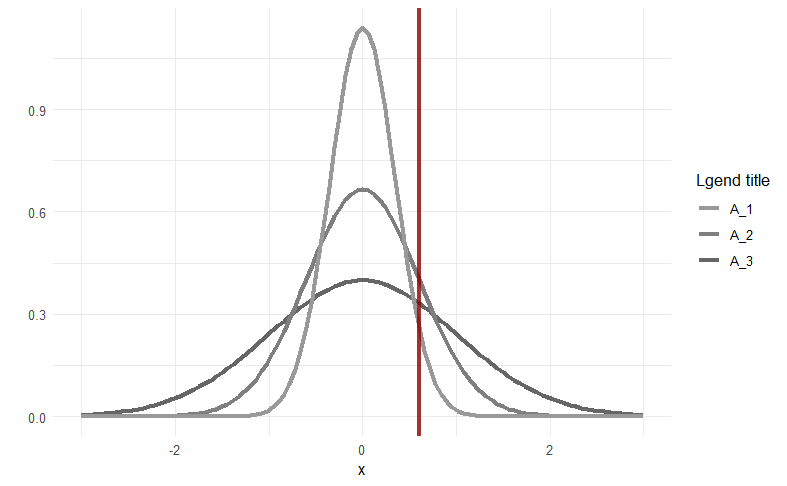
\includegraphics[width = .6\textwidth]{Figures/BNN_modelcheck.png}
    \caption{\footnotesize{Arbitrary representation of network generalizability, based on model complexity controlled by the number of hidden layers. Data within the central tendency of the red line may find the network with two hidden layers to be the most preferable}}
    \label{BNNmodelcheck}
\end{figure}

It would be interesting to compare specific architectures for the Tohoku Earthquake example, or any other appropriate example too.  Moving beyond, the application of Bayes to convolutional layers, specifically a comparison of probabilistic and deterministic models for high-level computer vision tasks, would be worth studying.


\subsection{Online Learning}
One can imagine scenarios in which the data is becoming available in real time, or even situations where a model is trained incrementally on data, as though it was fed through a hopper.  This makes especially interesting Bayesian techniques for online learning \cite{opper1999bayesian}, in which the BNN is trained in this way.  The Bayesian Updating rule would apply to cyclically recycle posteriors into priors in the presence of new data.  Further studies on this concept would be interesting to apply to practical application, such as in stock price fluctuation or weather prediction.

\subsection{BNN/ANN Regularizers}
It was noted several times that the assumptions of the prior distribution directly impact the BNN, specifically the recognizable regularization technique that its point-estimate correspondent would employ.  Literature \cite{vladimirova2019understanding} \cite{chiuso2016regularization} makes note of alternative priors and their coincidence with other regularization techniques (i.e. LASSO).  However, no publication exists based solely on the resemblance of probabilistic models with specific priors and their non-Bayesian counterparts.  It could be noteworthy to compare models built under each paradigm and demonstrate the level of engineering each would require as well as their predictive capabilities.

\bibliographystyle{unsrt}
\bibliography{ref}

\end{document}
